\apendice{Especificación de diseño}

\section{Introducción}

En este apartado detallaremos la arquitectura del proyecto centrandonos en aspectos fundamentales para el desarrollo de \textbf{VACA}. Se describira como se organizan los datos que lo componen, su diseño procedimental y la interconexión entre los objetos que conforman el sistema, con el objetivo de dar una vision técnica y detallada que justifique las decisiones que he adoptado durante la fase de desarrollo.

\section{Diseño de datos}

La aplicación \textbf{VACA} gestiona principalmente estos tipos de datos:

\begin{itemize}
    \item \textbf{Prompts de voz(Input):} capturados por un microfono porteriormente tratados y transformados a un formato \texttt{.wav}
    \item \textbf{Prompts en text(Input):} tratados directamente saltandose el paso de tratamiento de voz.
    \item \textbf{Representación textual gráfica:} tratado por los modelos YOLO y FLORENCE, capturados directamente del entorno gráfico del usuario.
    \item \textbf{Generación de logs:} Para mantenimiento del programa en caso de fallos guardados directamente en el sistema local del usuario.
\end{itemize}

La gran mayoria de datos se almacenan temporalmente en buffers y no persisten por motivos de privacidad, hay otros datos que se guardan en el propio sistema local para su tratamiento y posterior envio al servidor de ITCL.

Como se menciono con anterioridad el ITCL no guarda ni trata los datos que se reciben desde sus endpoints, ademas de ser datos volatiles, dado que los contenedores se eliminan una vez no esten en funcionamiento.

\section{Diseño arquitectónico}

El proyecto está diseñado para ser modular, facilitando la sustitución de componentes (por ejemplo, usar otro modelo STT o TTS) sin alterar el núcleo del sistema.

A continuación detallare el UML del sistema:

\begin{figure}[h!]
  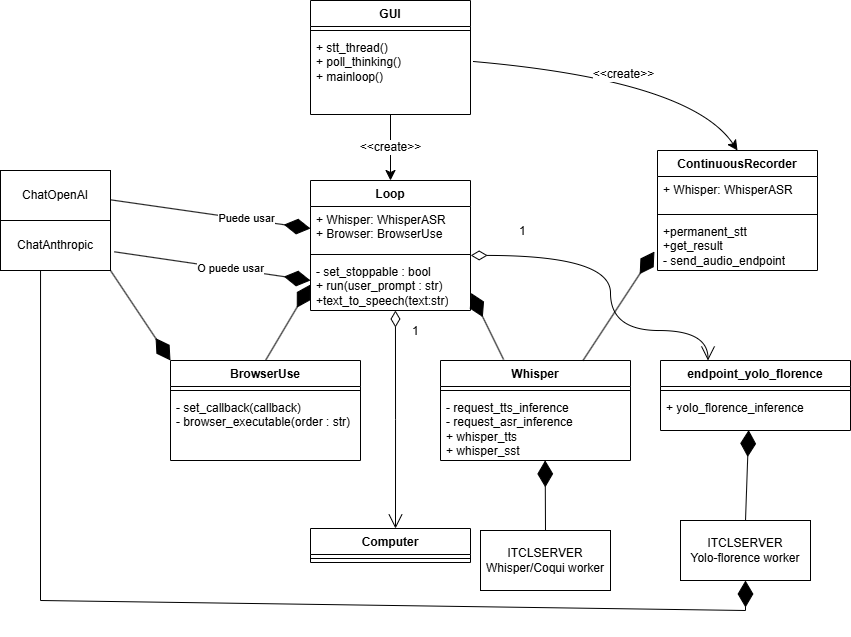
\includegraphics[scale=0.45]{img/Diagrama_clases.drawio.png}
  \caption{Diagrama de clases UML}
  \label{fig:UML}
\end{figure}

\subsection{Explicación de clases}
\begin{itemize}

    \item \textbf{GUI:} Representa la interfaz principal del programa, crea el Loop y hace uso de \texttt{ContinuousRecorder} para realizar inferencia continua sobre el audio recibido.

    \item \textbf{Loop:} La clase central del agente. \texttt{Loop} está compuesta por \texttt{BrowserUse} y \texttt{Whisper}, ya que necesita de ambas para cumplir su funcionalidad principal. 
    
    También incorpora una composición con las librerías de LangChain (\texttt{ChatOpenAI} o \texttt{ChatAnthropic}), siendo estas imprescindibles para el funcionamiento del sistema, aunque solo una puede estar activa en tiempo de ejecución.
    
    Adicionalmente, mantiene una dependencia con \texttt{endpoint-yolo-florence}, que permite la comprensión del contexto visual del entorno. Por último, \texttt{Loop} presenta una relación de agregación con el resto de herramientas de \texttt{Computer}, como escritura, movimiento de ratón, etc.

    \item \textbf{Whisper:} La clase \texttt{Whisper} tiene una composicion hacia \texttt{ContinuousRecorder} y \texttt{Loop}, ya que ambas dependen de ella para ejecutar funciones vitales. Estas funciones incluyen la transcripción continua del audio (STT) y la generación de archivos \texttt{.wav} con las respuestas del agente (TTS).
    
    Si bien la parte de TTS podría desacoplarse y gestionarse directamente desde \texttt{Whisper}, se ha optado por mantener esta responsabilidad dentro de \texttt{Loop}, dado que actúa como el núcleo del agente.
    
    Aunque esta implementación genera una composición fuerte, \texttt{Whisper} ha sido diseñada para realizar peticiones a un servidor externo del ITCL. Esto permite una cierta flexibilidad: para cambiar el modelo de inferencia (TTS/STT), solo sería necesario modificar el endpoint correspondiente dentro de \texttt{Whisper}, siempre y cuando el nuevo modelo siga utilizando los mismos formatos de entrada y salida.
    
    \item \textbf{BrowserUse:} Aunque no es estrictamente necesaria para el funcionamiento del agente, ya que algunas herramientas internas de \texttt{Computer} pueden cubrir parcialmente sus funciones, se ha optado por incluirla mediante composición dentro de \texttt{Loop}, ya que mejora considerablemente la precisión en las tareas de búsqueda.
    
    Cabe mencionar que \texttt{BrowserUse} depende completamente de \texttt{ChatAnthropic} para su funcionamiento, por lo que no puede operar sin esta.

    \item \textbf{ContinuousRecorder:} Aunque \texttt{GUI} no está compuesta directamente por esta clase ,debido a que existen funciones alternativas (actualmente desactivadas) para la transcripción, \texttt{ContinuousRecorder} representa un módulo importante dentro de la interfaz.
    
    Es responsable de la captura de audio y su conversión continua a texto sin interrupciones. Esta clase depende totalmente de \texttt{Whisper}, ya que sin ella no puede realizar las transcripciones.

    \item \textbf{endpoint-yolo-florence:} Al igual que \texttt{ContinuousRecorder}, este componente es esencial para ciertas funcionalidades de \texttt{Loop}, particularmente para la comprensión del contexto visual.
    
    No obstante, el agente puede seguir funcionando parcialmente sin él, motivo por el cual se ha modelado como una agregación y no como una composición directa desde \texttt{Loop}.

    \item \textbf{Computer:} Incluye herramientas auxiliares utilizadas por \texttt{Loop}, tales como el movimiento del ratón, escritura mediante teclado, y otras funcionalidades relacionadas con el control del sistema operativo.

    \item \textbf{ChatOpenAI / ChatAnthropic:} Son las interfaces que permiten interactuar con modelos de lenguaje a través de LangChain. Constituyen una parte fundamental del sistema, ya que sin ellas el agente no podría generar respuestas ni mantener una conversación.

    \item \textbf{ITCLSERVER Whisper / Coqui:} Corresponden a los modelos de inferencia TTS/STT alojados en los servidores del ITCL. Son utilizados por la clase \texttt{Whisper} para procesar el audio recibido (transcripción) o generar audio a partir de texto.
    
    \item \textbf{ITCLSERVER YOLO / Florence:} Contienen los modelos de visión por computador encargados de detectar objetos y generar una representación gráfica del entorno. La lógica actual de estos modelos está acoplada a \texttt{ChatAnthropic} para obtener descripciones semánticas, aunque esta parte podría desacoplarse fácilmente y ubicarse directamente dentro de \texttt{endpoint-yolo-florence}.
    
    Esto permitiría que el endpoint devuelva un diccionario de índices, coordenadas, descripciones y una imagen procesada ("yoleada"), facilitando así una mayor modularidad. Sin embargo, por motivos de simplicidad y comodidad, se ha mantenido la lógica actual en el worker.

\end{itemize}

\subsection{Diseño centrado en la clase Loop}
Durante el desarrollo del agente, se tomó la decisión de estructurar el sistema de forma que la clase \texttt{Loop} actuase como el núcleo central de la aplicación. Esta elección responde a la necesidad de contar con un componente que coordinara de forma ordenada todas las funcionalidades críticas del sistema: procesamiento de lenguaje natural, transformacion de audio a texto, percepción visual del entorno, interacción con herramientas del sistema operativo y uso de fuentes externas como navegadores.

\texttt{Loop} se encarga de realizar la ejecución del agente, controlando cuándo y cómo deben actuar los distintos módulos. Por esta razón, se le asignaron relaciones de composición con elementos esenciales como \texttt{Whisper} (para STT y TTS), \texttt{BrowserUse} (búsqueda en la web), y las librerías de LangChain (\texttt{ChatOpenAI} o \texttt{ChatAnthropic}), ya que su funcionamiento correcto depende directamente de estos para llevar a cabo su lógica y función principal.

Adicionalmente, \texttt{Loop} mantiene relaciones de agregación con componentes más secundarios, como los módulos de visión (\texttt{endpoint yolo-florence}) o las herramientas de \texttt{Computer} (teclado, ratón, etc.), permitiendo que estas puedan activadas o desactivadas sin comprometer la integridad del sistema.

Aunque esta centralización puede dar lugar a una clase con muchas responsabilidades, lo que en ingeniería del software se conoce como un "God Object", en este caso se justifica plenamente por el contexto del proyecto. Al tratarse de un agente que debe operar de manera autónoma y reactiva, resulta conveniente contar con un único punto de entrada que mantenga el control y secuenciación de los diferentes módulos.

Además, este diseño permite una clara separación entre el núcleo lógico del agente y sus módulos funcionales. Cada clase ha sido diseñada para tener responsabilidades bien delimitadas, permitiendo que su lógica interna se mantenga lo más independiente posible. Esta modularidad facilita la sustitución de componentes individuales (por ejemplo, cambiar el modelo de lenguaje o el motor de transcripción) sin necesidad de alterar el diseño general del sistema.

\subsubsection{Conclusion}
He priorizado un enfoque que combina centralización lógica en \texttt{Loop} con una arquitectura modular, en la que cada componente mantiene un alto grado de cohesión. Esta estructura no solo facilita el mantenimiento y la escalabilidad futura del proyecto, sino que también hace más clara su comprensión y evaluación.

\section{Diseño procedimental}

En este apartado describire la lógica del flujo de trabajo del sistema relacionado con las tareas principales de la aplicación.


\begin{enumerate}
\item La clase \texttt{GUI} inicia la ejecución del programa y lanza un bucle continuo gestionado por la clase \texttt{Loop} para inicializar el CUA.

\item \texttt{Loop} activa el contenedor de \texttt{Whisper}, que emplea \texttt{ContinuousRecorder} para comenzar la captura y transcripción continua de audio.

\item Cuando se detecta un prompt de voz, se valida la entrada y se encapsula como un prompt. En caso de hacer una introducción por teclado simplemente habría que escribir el prompt y enviarlo.

\item El prompt es analizado por el modelo LLM (a través de \texttt{ChatOpenAI} o \texttt{ChatAnthropic}) para extraer la intención del usuario.

\item Si el LLM determina que necesita información visual, se activa el endpoint \texttt{yolo-florence}, que genera una descripción semántica del entorno gráfico.

\item Si la tarea requiere datos externos, \texttt{BrowserUse} lanza una búsqueda web y filtra los resultados obtenidos.

\item Una vez recolectada toda la información necesaria (contexto visual, datos externos, historial, etc.), el agente genera una respuesta textual, que se muestra al usuario a través de la interfaz \texttt{GUI}.

\item En caso de ser necesario para cumplir la intención del usuario, el agente utilizaría herramientas incorporadas para conseguir el objetivo descrito por el usuario.

\item Opcionalmente, la respuesta puede ser vocalizada. Para ello, \texttt{Loop} reutiliza \texttt{Whisper} para convertir el texto en audio mediante TTS, el cual se reproduce automáticamente.

\item Finalmente, el agente queda de nuevo en espera de una nueva interacción, reiniciando el ciclo.
\end{enumerate}

A continuación se mostrara el diagrama de secuencia de todas las tareas mencionadas anteriormente.

\begin{figure}[h!]
  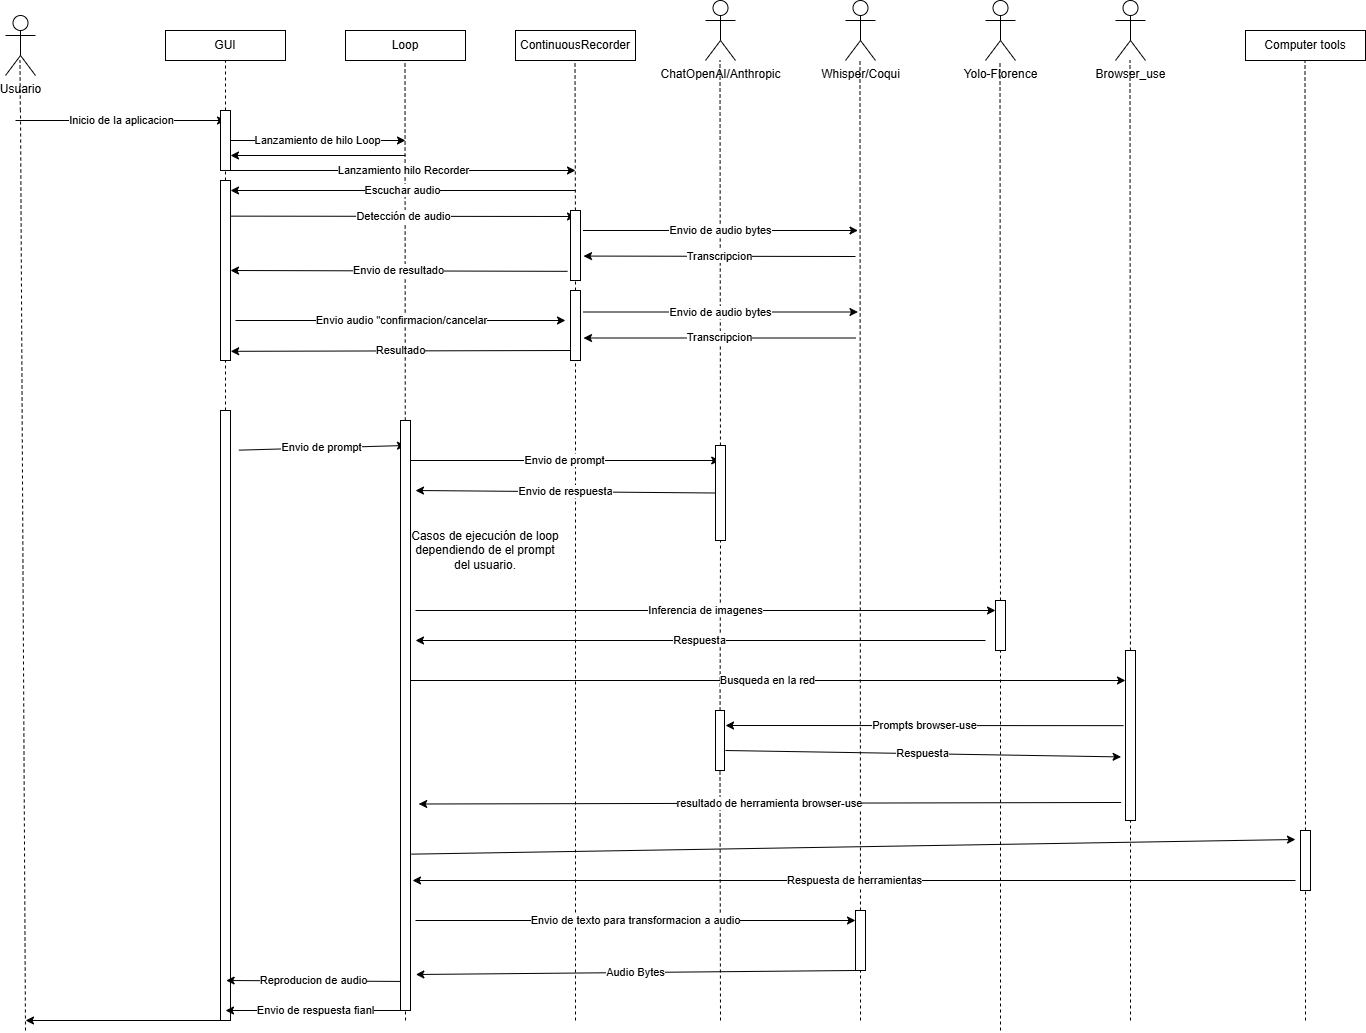
\includegraphics[scale=0.35]{img/Diagrama secuencia.drawio.png}
  \caption{Diagrama de secuencia de todas las tareas.}
  \label{fig:UML}
\end{figure}